\documentclass{subfiles}

\begin{document}
	\begin{figure*}[htp]
		\centering
		\subfloat{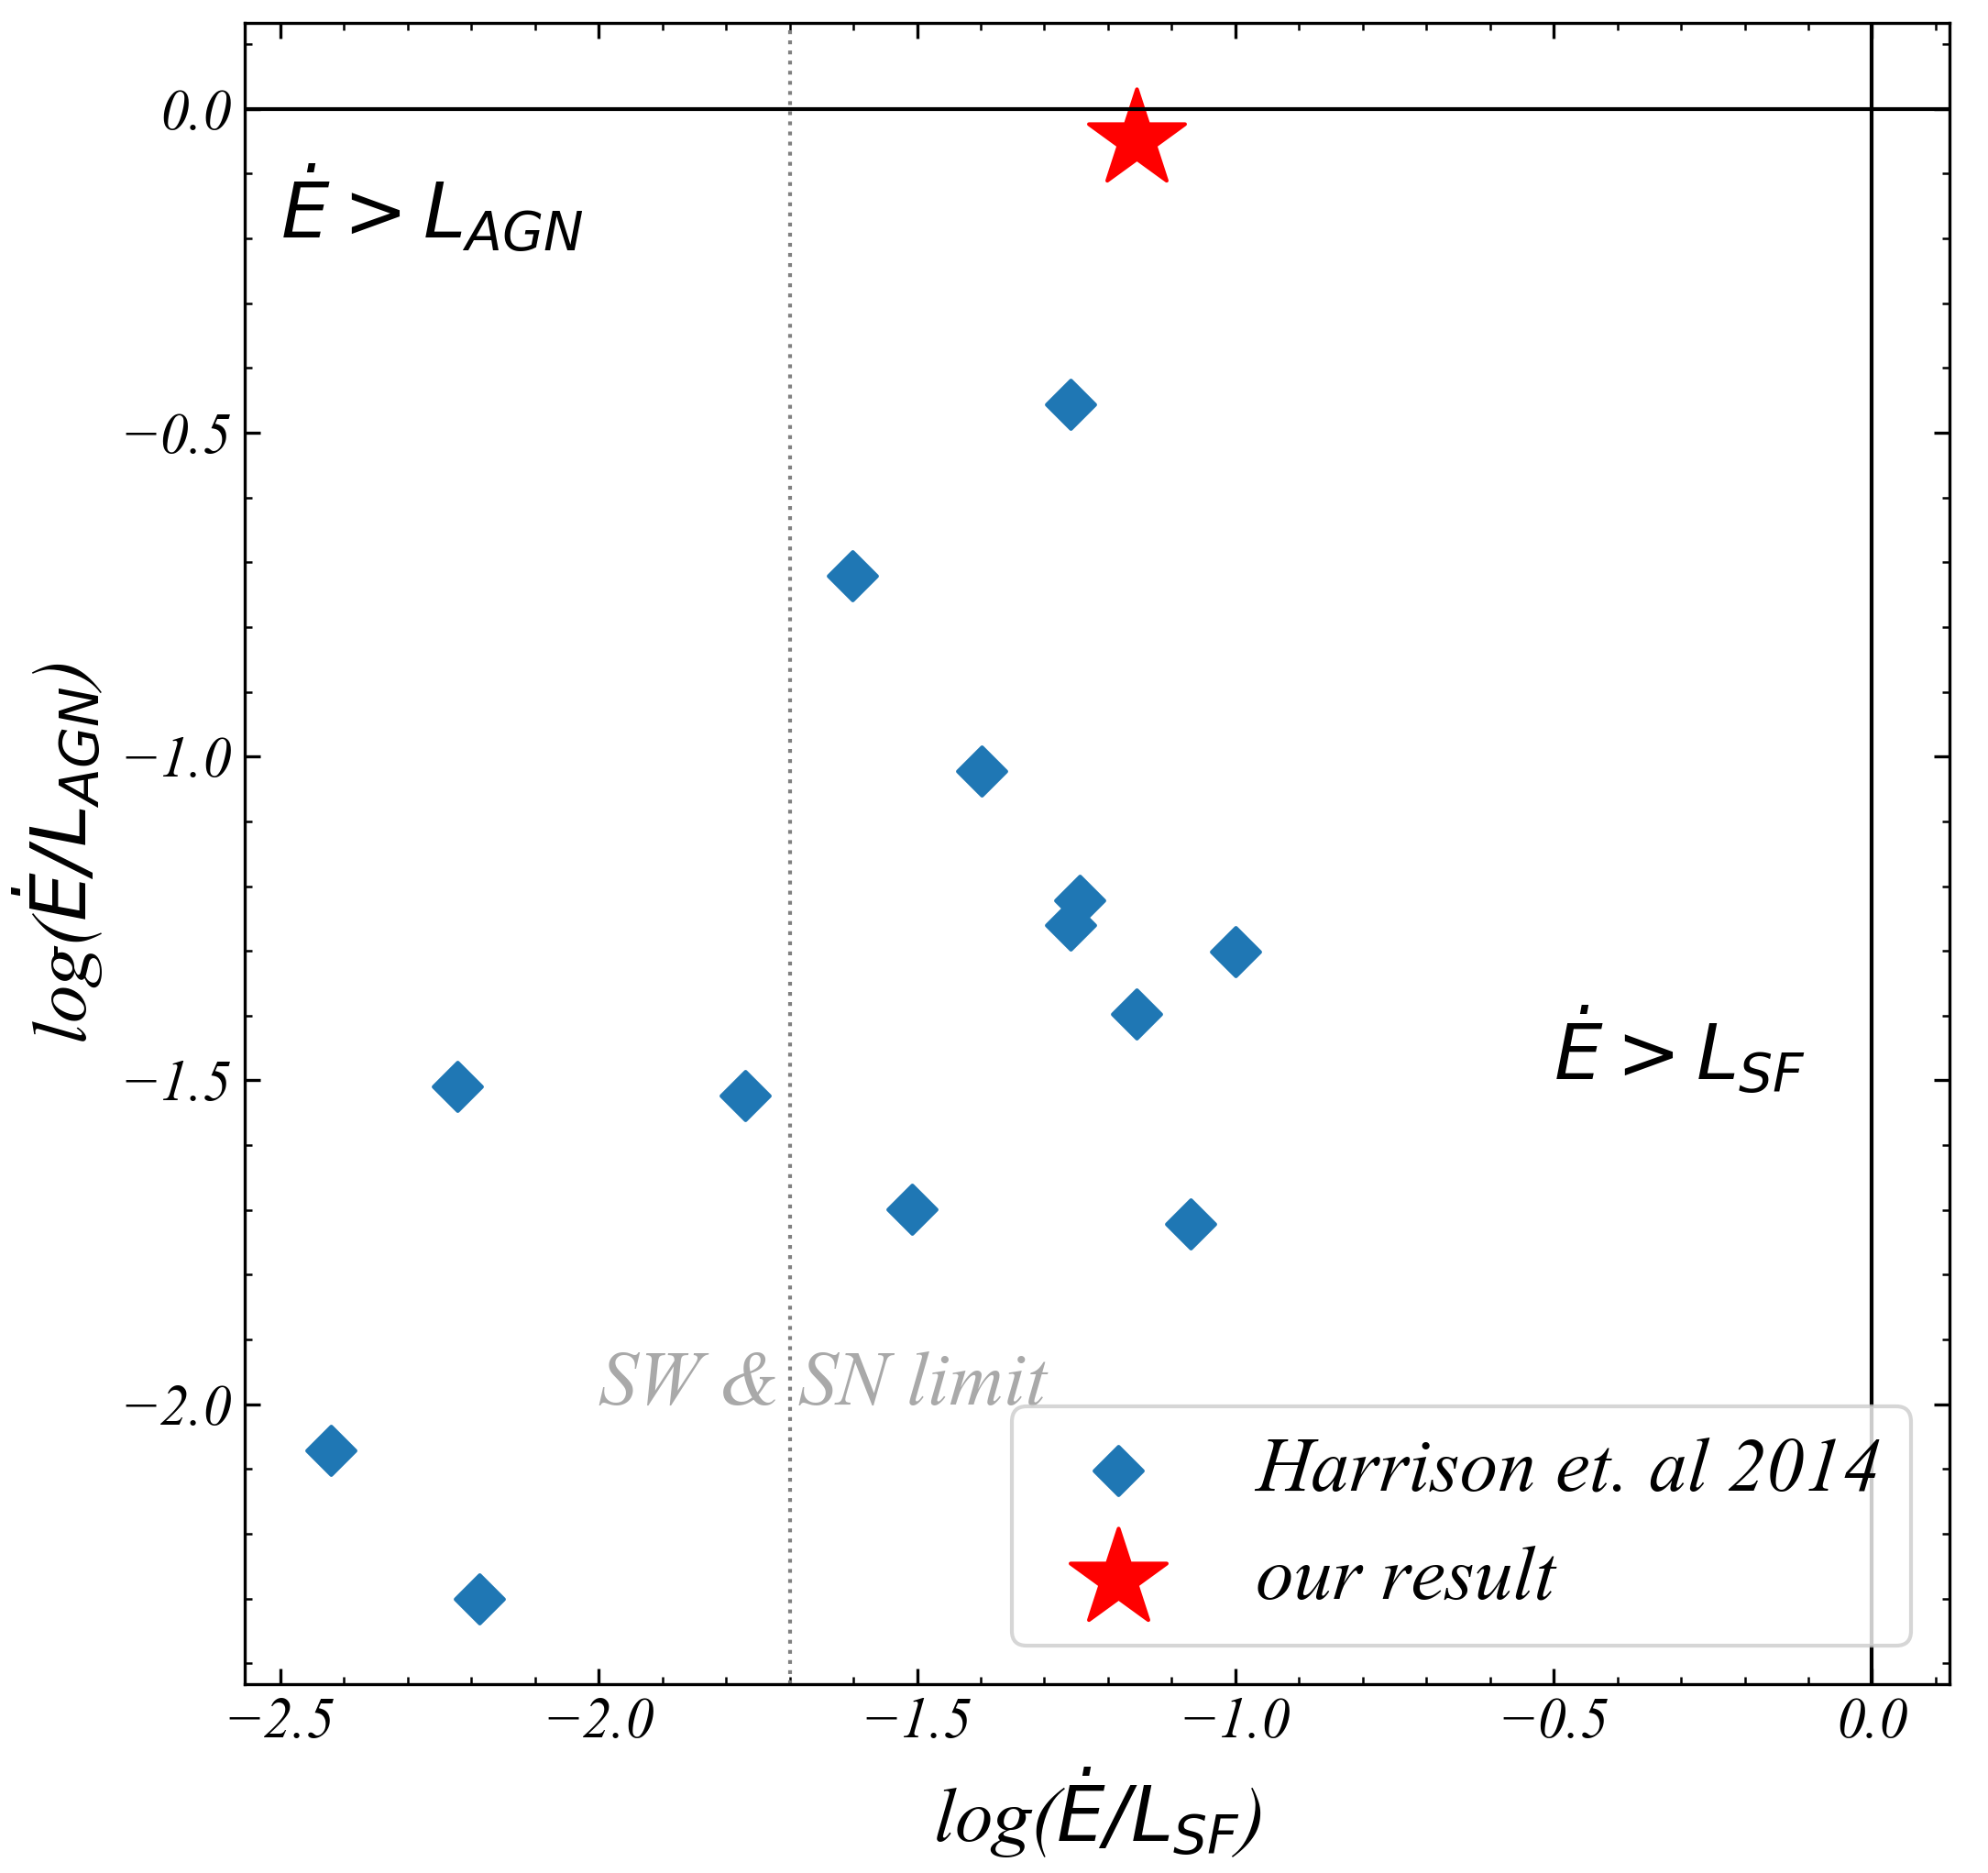
\includegraphics[width=0.5\textwidth]{figs/cp_AGN_vs_cp_SF}}
		\subfloat{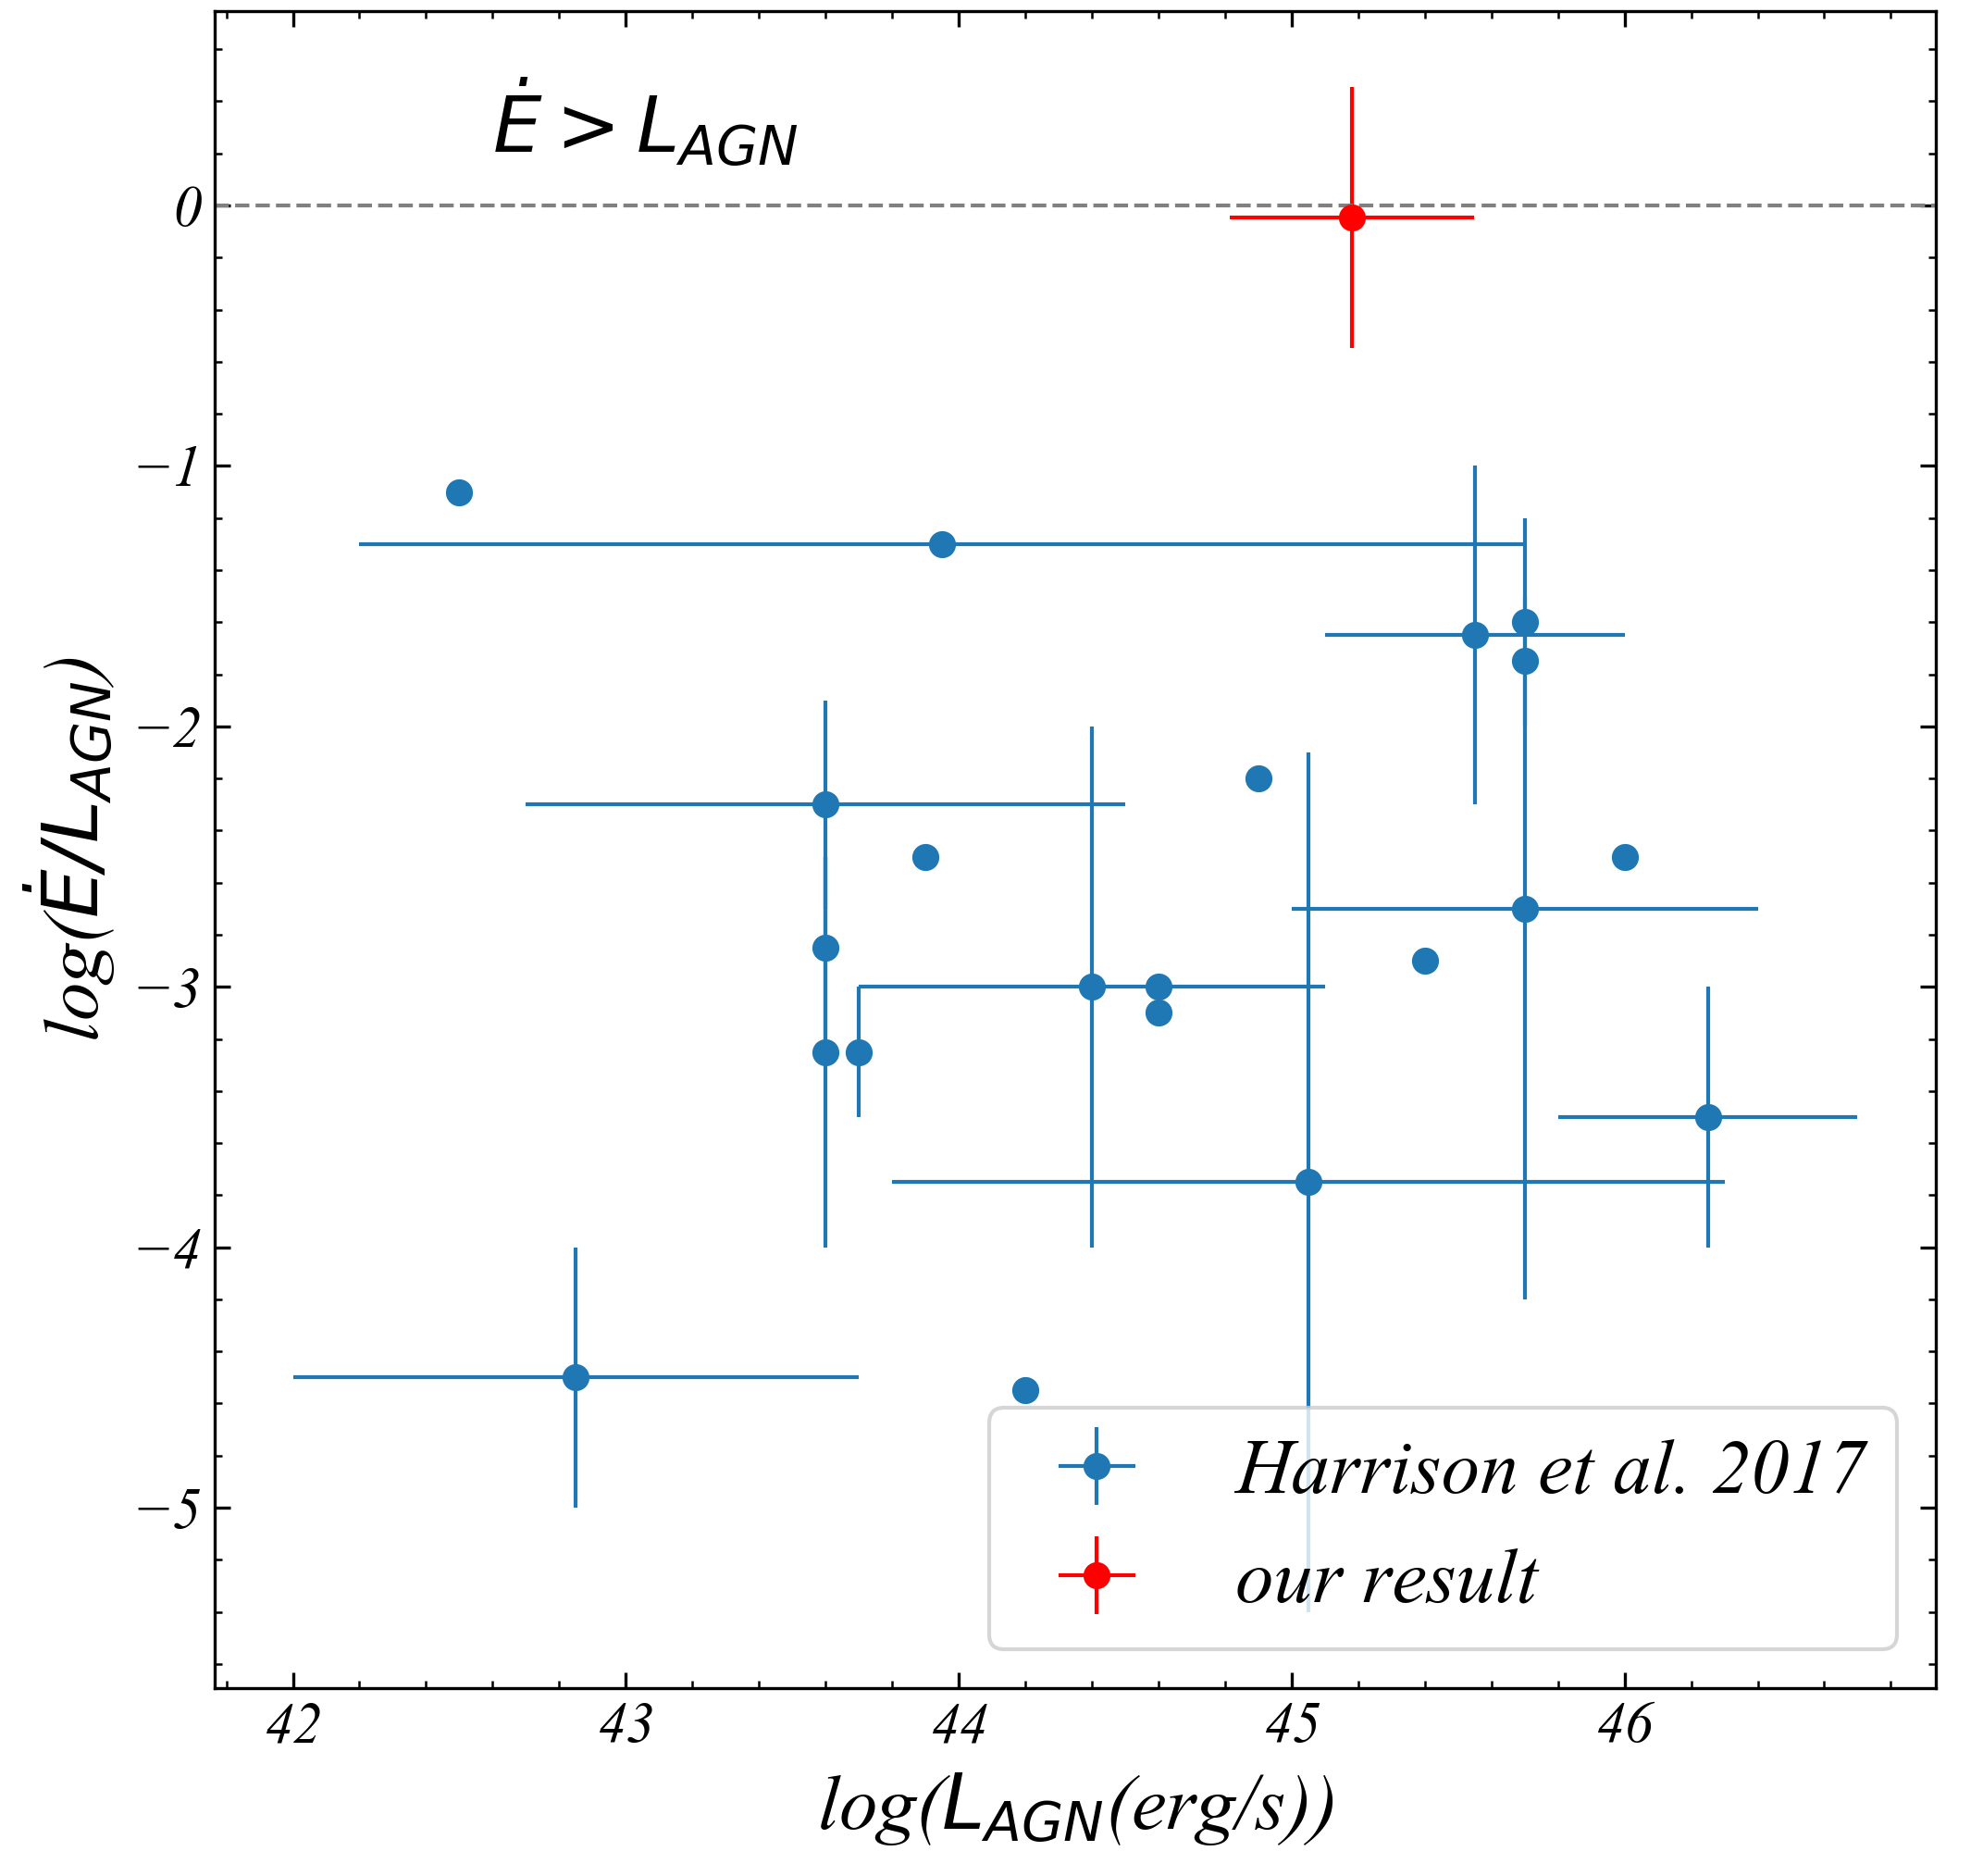
\includegraphics[width=0.5\textwidth]{figs/cp_AGN_vs_L_AGN}}
		\label{coupeffic}
		\caption{Left: the ratio of our estimated outflow kinetic energy rates($E_{out}$) to the AGN luminosity and to the star formation luminosity for our source(red) and sources from \cite{harrison2014kiloparsec}. The dashed vertical line is the estimated maximum mechanical input expected from supernovae and stellar winds. The two solid lines shows the coupling efficiency of 1. Right: Observationally determined kinetic coupling efficiencies in \cite{harrison2018agn} and our result. The vertical lines show the range of values quoted or, in the case of an error bar, the quoted error on the average value. The horizontal lines show the range of bolometric luminosity for each sample. The dotted line shows coupling efficiency of 1. }
	\end{figure*}
	
	In this section we will investigate which of these processes could responsible for driving the extreme outflows observed. The dominant processes that drive such large scale outflow in protocluster and the efficiency to which they are able to couple the gas are currently sources of uncertainty in galaxy formation models. Several possible mechanisms have been suggested to drive galaxy-wide outflows, for example: the stellar wind and supernovae; radiation pressure from the extremely luminous AGN or star formation; the interaction of radio jets with a clumpy and multiphase interstellar medium; AGN wind initially launched from the accretion disc. Following \cite{harrison2014kiloparsec}, we calculate the coupling efficiency which is a popular method to investigate the likely drivers of large-scale outflow. We compare the ratio of our outflow kinetic energy rate($\dot{E_{out}}$) with (1) the FIR AGN luminosity; (2) the FIR star formation luminosity (these two power are given by \cite{arrigoni2018qso}). We also calculate the momentum-loading factor for both star-forming-driven case and AGN-driven case. Using these results we now explore the possible driving mechanisms to power this outflow. 
	 
	 Fig.\ref{coupeffic} shows coupling efficiency for both star-forming-driven case and AGN-driven case. We compare our result with results in \cite{harrison2014kiloparsec}. One way for star formation to drive large-scale outflow is by stellar winds or supernovae. An estimation of the coupling efficiency for this case is carried by \cite{kennicutt1998star}, he found that the maximum coupling efficiency is $\dot{E_{out}}/L_{IR,SF} \approx 0.02$, we indicate this upper limit with gray dot line in Fig.\ref{coupeffic}. Based on this results, stellar winds and supernovae are unlikely to be fully responsible for the observed outflows. On the other hand, the coupling efficiency for AGN-driven case is too large which is close to 1. In the right panel of Fig.\ref{coupeffic} it shows that if the outflow is driven by AGN, it has already exceed other results with similar AGN luminosity. 
	 
	 Besides, if we instead consider a momentum-driven wind with momentum deposition from the radiation pressure of stars or AGN, the momentum loading factor $f_{p}=log(c\dot{P_{out}}/L)$ is $f_{p,SF}=1.7$ and $f_{p,AGN}=3.2$ respectively. Nevertheless \cite{zubovas2018agn} suggests that a typical momentum loading factor for star-formation-driven case is $f_{p,SF}< 1.4$ which is lower than our estimation, this comparison also rules out the star-formation case. In the same way, we also find that $f_{p,AGN}$ is larger than the typical value. 
	 
	 Moreover, \cite{shankar2006new} mentions the two sources of feedback are important over different mass ranges, in particular, stellar feedback regulates the processes in low-mass galaxies while large galaxies are mainly regulated by AGN feedback. The transition mass for this two feedback mechanisms is $M_{tr} \approx 2 \times 10^{10} \mathrm{M}_{\odot} $. By fitting the SED of source-B, \cite{arrigoni2018qso} estimates its stellar mass of source-B to be $\log \left(M_{\mathrm{star}} / \mathbf{M}_{\odot}\right)=11.4_{-0.2}^{+0.3}$. Comparing with $M_{tr}$, this results also suggests that feedback from star formation is not the dominant reason for the outflow.  
	 
	 However, \cite{zubovas2018agn} also suggests there are mechanisms to reach high coupling efficiency and momentum loading factor. One possibility is hyper-Eddington SMBH growth during Compton-thick(heavily obscured) phases. In this case, SMBH would accrete material with extremely large rate and may lead to ultra fast outflows(UFO).  \cite{tombesi2013unification} shows that this outflow can reach the velocity $\approx 0.1c$ and will have a strong coupling with the interstellar medium(ISM). Fig.6 of  \cite{tombesi2013unification} shows some coupling efficiency of some UFOs $\approx 1$, but he also explains that this extremely fast and powerful outflow would occur only very close to SMBH $R \approx 1000r_{s}$(where $r_{s}$ is the schwarzschild radius.).  He indicates that the large coupling efficiency is probably due to large environment column density $\approx 10_{24} cm^{-2}$ and highly ionized state. These two factors are consistent with the large-scale environmental conditions(MAMMOTH-1, extreme onverdensities; enomous lyman$\alpha$ nebula.). Nevertheless, \cite{cai2017discovery} suggests that the hydrogen column density is in the range $\approx 10^{20} cm^{-2}$, we indicate here that the column density in CGM maybe $10^{3} cm^{-2}$ larger than this value. 
	 
	 In summary, based on our analyses we find the outflow is unlikely powered by star-forming processes, but we do see some similar behaviors between the outflow and UFO(high coupling efficiency and high momentum loading factor), so we conclude that this outflow maybe driven by accretion-disc winds. Although there's large uncertainty coupling efficiency estimation, this large coupling efficiency and momentum loading factor have never been seen on such a large scale. From the observation it's still unclear what kind of mechanism leads to such large coupling efficiency on such large scale(the typical coupling efficiency beyond 10kpc <0.01), it maybe results from large column density $>10^{24}cm^{-2}$ or very efficient cooling mechanism. Besides, it provides evidence that outflow from central quasar can truely have influence on the protocluster.

\end{document}